\documentclass[../main.tex]{subfiles}
\graphicspath{
    {"../img/"}
    {"img/"}
}

\begin{document}
    Ostatnio było:
    \begin{align*}
        &A\subset D : \underset{x\in A}{\forall} \mathcal{O}(f,x)<\varepsilon; A - \text{kostka, to}\\
        &\underset{\Pi}{\exists} | \overline{S}(f,\Pi) - \underline{S}(f,\Pi)| < \varepsilon |A|
    .\end{align*}
    \begin{tw}
        (Lebesgue'a) niech $D$ - kostka, $D\subset \mathbb{R}^n$, $f: D\to \mathbb{R}$, $f$ - ograniczona.\\
        Wówczas $f$ - (całkowalna na $D$ ) $\iff$ (zbiór nieciągłości funkcji $f$ jest miary Lebesgue'a zero)
    \end{tw}
    \begin{dowod}
        $\impliedby$ \\
        Chcemy pokazać, że \[
            \underset{\Pi}{\exists} |\overline{S}(f,\Pi) - \underline{S}(f,\Pi) | < \varepsilon
        ,\]
            \begin{figure}[h]
                \centering
                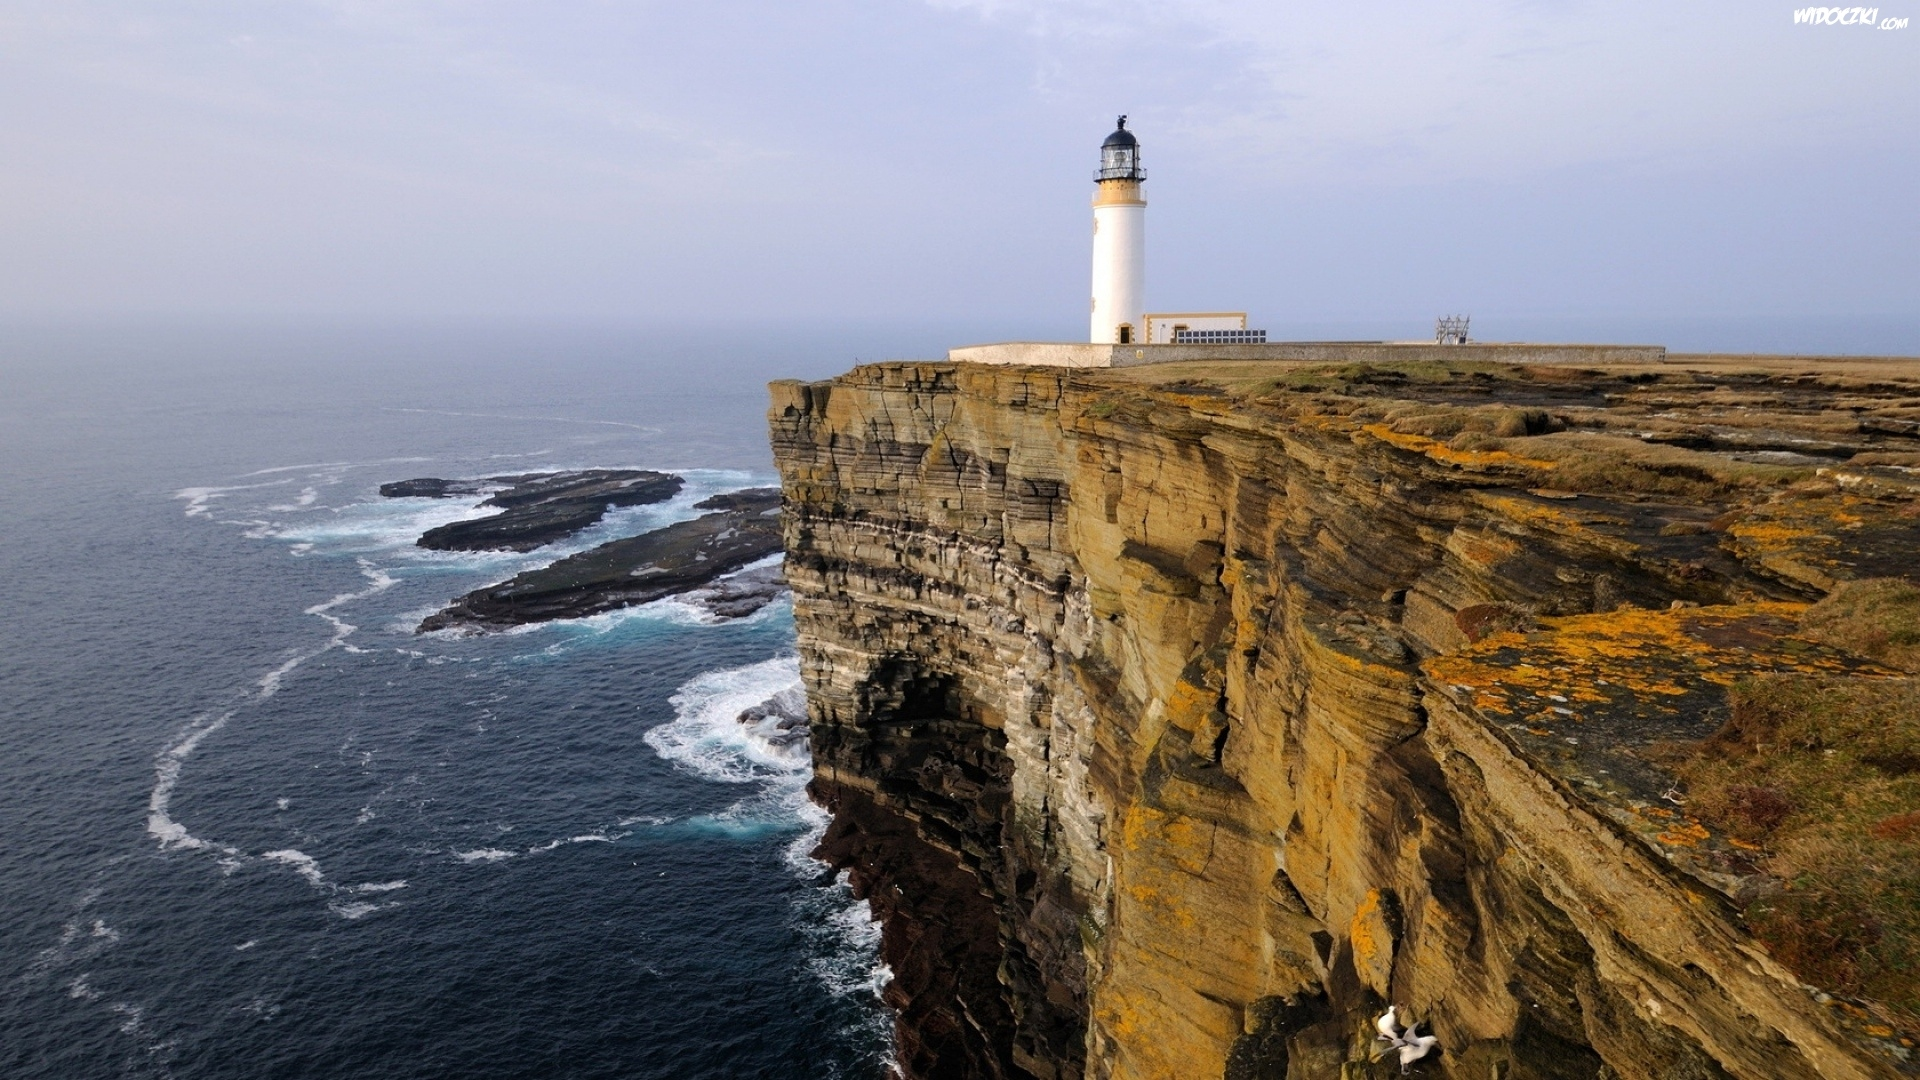
\includegraphics[width=0.8\textwidth]{fig_41}
            \end{figure}
        przy założeniu, że zbiór nieciągłośći jest miary L. zero.\\
        Wprowadźmy zbiór $A_n = \left\{ x\in D, \mathcal{O}(f,x) \ge \frac{1}{n} \right\} $
        \[
            \text{np. } A_2 = \left\{ x\in D, \mathcal{O}(f,x) \ge \frac{1}{2} \right\}
        .\]
        \begin{obserwacja}
            $A_1\subset A_2\subset A_3\subset \ldots$\\
            a zbiór $A = \bigcup_{n=1}^{\infty}A_n$ będzie zbiorem wszystkich punktów nieciągłości funkcji $f$ na  $D$.\\
        \end{obserwacja}
            Tw. Lebesgue'a udowodnimy dla wybranego $A_n$, bo przeliczalna suma zbiórów miary L. zero też jest zbiorem miary L. zero.
        \begin{uwaga}
            Zbiór $A_n$ jest zbiorem domkniętym (bo lemat).\\
            Wiemy, że $A_n$ jest zbiorem miary L. zero gdy itnieje $P_i \subset D$, ($P_i$ - kostki), że $A_n \subset \bigcup P_i $, $\sum |P_i |$ - dowolnie mała (skończona lub nieskończona suma).\\
        \end{uwaga}
        Niech $\varepsilon > 0$. Wiemy, że
        \[
        \underset{\varepsilon>0}{\forall} . \underset{N}{\exists} . \underset{n > N}{\forall} \frac{1}{n} < \varepsilon
        .\] Wybierzmy zatem taki indeks $n$ dla zbioru $A_n$, że $\frac{1}{n} < \varepsilon$.
        Wiemy, że $A_n$ - domknięty i ograniczony (bo $A_n \subset D$, a $D$ - kostka w $\mathbb{R}^n$), to znaczy, że $A_n$ jest zbiorem zwartym, a $\left\{ P_i \right\} $ jest jego pokryciem.
        Możemy więc wybrać z niej skończone podpokrycie $\left\{ P_1, P_2, \ldots, P_k \right\} $ takie, że
        \begin{align*}
        &A_n \subset \bigcup_{j=1}^k P_j\\
        &\sum_{j=1}^{k} |P_j| < \frac{1}{n}
        .\end{align*}
        (możemy tak zrobić, bo zawsze możemy wybrać taką rodzinę $\left\{ P_i \right\} $, że $\sum |P_i|$ - dowolnie mała.
        \begin{figure}[h]
            \centering
            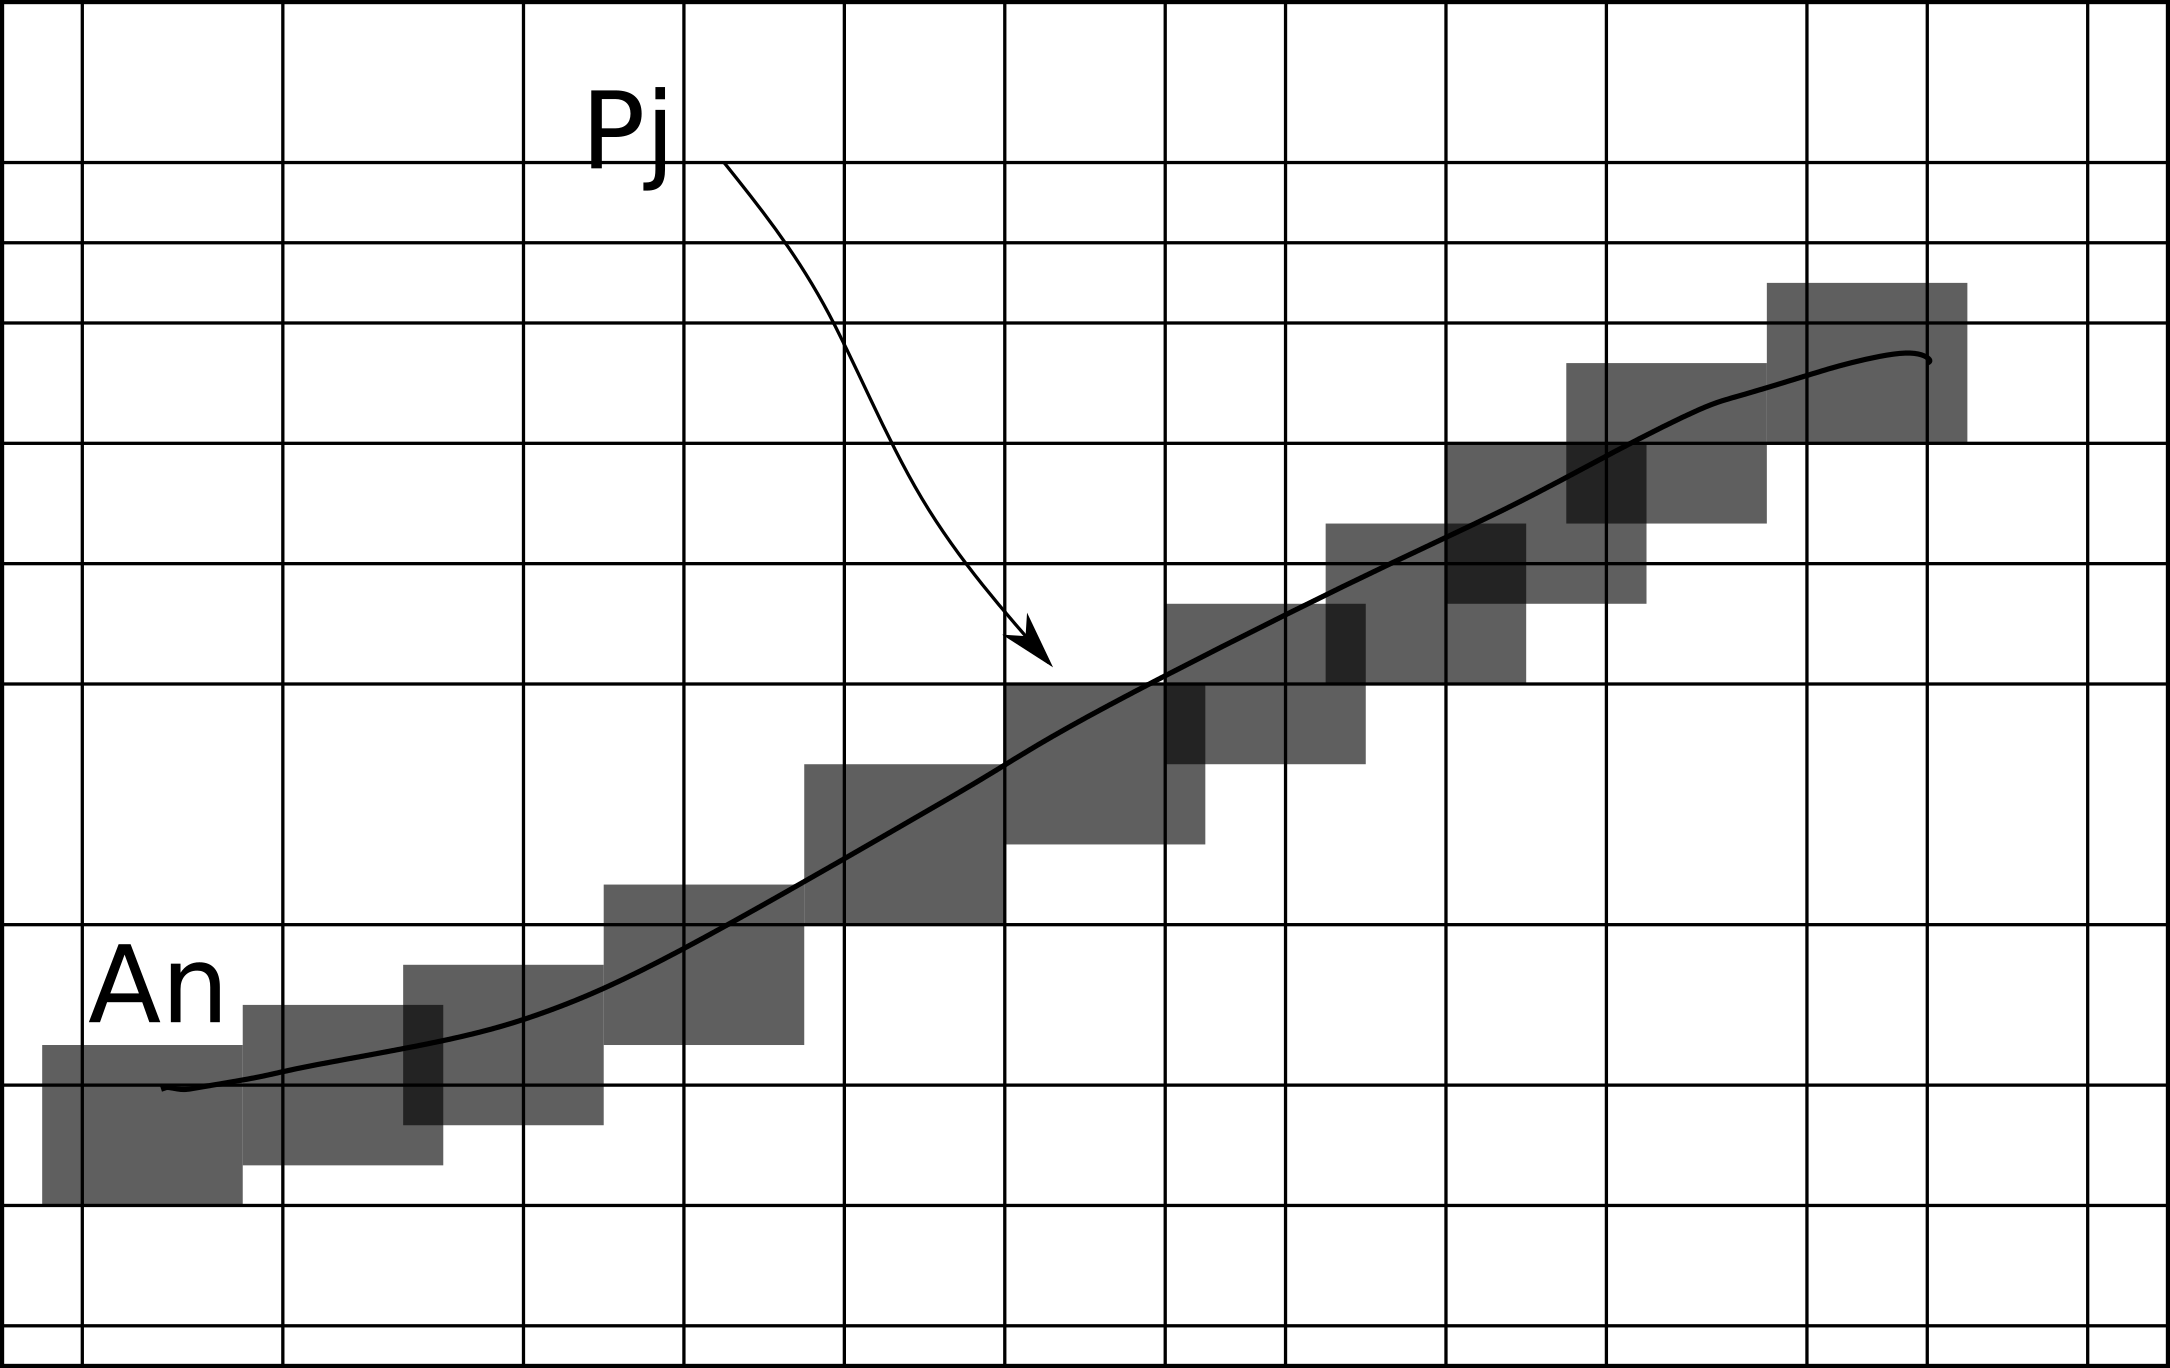
\includegraphics[width=0.8\textwidth]{fig_42}
        \end{figure}
        Wybierzmy podział $\Pi$ zbioru $D$ taki, że $\Pi$ jest na tyle drobny, że odtwarza pokrycie $A_n$ zbioru $\bigcup P_j$. Oznacza to, że podział $\Pi$ możemy podzielić na dwa podziały
        \begin{align*}
            &\Pi = \Pi_1 \cup \Pi_2 \text{, takie że}\\
            &\Delta\\
            &\Pi_1 \cap \left\{ \bigcup_{j} P_j \right\} \neq \phi\\
            &\text{oraz } \Pi_2 \cap \left\{ \bigcup_{j} P_j \right\} = \phi
        .\end{align*}
        $\Delta$ : każda kostka z $\left\{ P_j \right\} $ składa się z kostek należących do $\Pi_1$

        $|\overline{S}(f,\Pi) - \underline{S}(f,\Pi)| = |\overline{S}(f,\Pi_1) - \underline(f,\Pi_1) + \overline{S}(f,\Pi_2) - \underline{S}(f,\Pi_2)|$, ale
        \begin{equation}\label{eq:Q}
            \overline{S}(f,\Pi_1) - \underline{S}(f,\Pi_1) = \sum_{Q_i\in\Pi_i}(\underset{x\in Q_i}{sup} f - \underset{x\in Q_I}{inf} f) Q_i |
        \end{equation}
        Gdzie wiemy, że $\sum |Q_i| < \frac{1}{n}$, a $f$ - ograniczona na $D$ czyli
        \[
            \underset{M}{\exists} .\underset{x\in D}{\forall} |f(x)| < \frac{M}{4}
        .\] Czyli
        \[
        |\underset{x\in D}{\sup} f - \underset{x\in D}{\inf} f | < M
        .\] Zatem
        \[
            \text{(\ref{eq:Q})} \le M \cdot \sum |Q_i| \le M \cdot  \frac{1}{n}
        .\]
        Ale
        \begin{align*}
            &\overline{S}(f,\Pi_2) - \underline{S}(f,\Pi_2) = \sum_{R_j \in \Pi_2}(\underset{x\in R_j}{\sup} f - \underset{x\in R_j}{\inf} f) |R_j|\\
            &\le \frac{1}{n} \sum |R_j| \le \frac{1}{n} |D|
        .\end{align*}
        Zatem
        \[
            |\overline{S}(f,\Pi) - \underline{S}(f,\Pi) \le M \cdot \frac{1}{n} + \frac{1}{n} |D| = \frac{1}{n} \cdot  const
        .\]
        czyli możemy tak zwiększyć $n$, że $\underset{\varepsilon>0}{\forall} \frac{1}{n}\cdot const < \varepsilon \quad\Box$\\
        Dlaczego wynika z tego prawdziwość dowodu dla całego $A$?\\
        np. dla $A_{2019}$ działa, ale co dalej. Bo $A_k$ dla $k>n$ też spełniają warunek, że $\frac{1}{k}\cdot const < \varepsilon$, a $A_j$ dla $j<n$ jest takie, że $A_j \subset A_n$

        $\implies$\\
        Wiemy, że $f$ - całkowalne, czyli
        \[
            \underset{\varepsilon>0}{\forall} . \underset{\Pi}{\exists} |\overset{S}(f,\Pi) - \underset{S}(f,\Pi) | < \varepsilon / n
        .\] (chcemy pokazać, że $A_n$ jest zbiorem miary L. zero)

        \begin{align*}
            &\Pi = \left\{ T_i \right\}\\
            &\frac{\varepsilon}{n} > |\overline{S}(f,\Pi) - \underline{S}(f,\Pi)| = \\
            &\sum | \underset{x\in T_i}{\sup} f - \underset{x\in T_i}{\inf} f| |T_i|
            (*)
        .\end{align*}
        z podziału $T_i$ wybieram takie kostki $P_i$, że $|\underset{x\in P_i}{\sup} f - \underset{x\in P_i}{\inf} f \ge \frac{1}{n}$.\\
        Wówczas
        \begin{align*}
            &(*) \ge \sum_{P_i} \frac{1}{n} | P_i | = \frac{1}{n} \sum |P_i|\\
            &\text{czyli } \underset{\varepsilon>0}{\forall} \frac{\varepsilon}{n} > \frac{1}{n} \sum |P_i|\text{, gdzie $P_i$ jest pokryciem $A_n$}
        .\end{align*}
        Czyli $A_n$ jest zbiorem miary L. zero $\quad\Box$
    \end{dowod}

    \begin{przyklad}
        $f(x,y) = x \sin(xy), \quad A=[0,1]\times[0,1]$\\
        $\int_A f \overset{\text{?}}{=} \int_{0}^{1} \varphi_1(x)dx \overset{\text{?}}{=} \int_0^1 \varphi_2(y)dy$,\\
        gdzie $\varphi_1(x) = \int_0^1 x\sin(xy)dy$, $\varphi_2(y) = \int_0^1 x\sin(xy)dx$
        \begin{figure}[h]
            \centering
            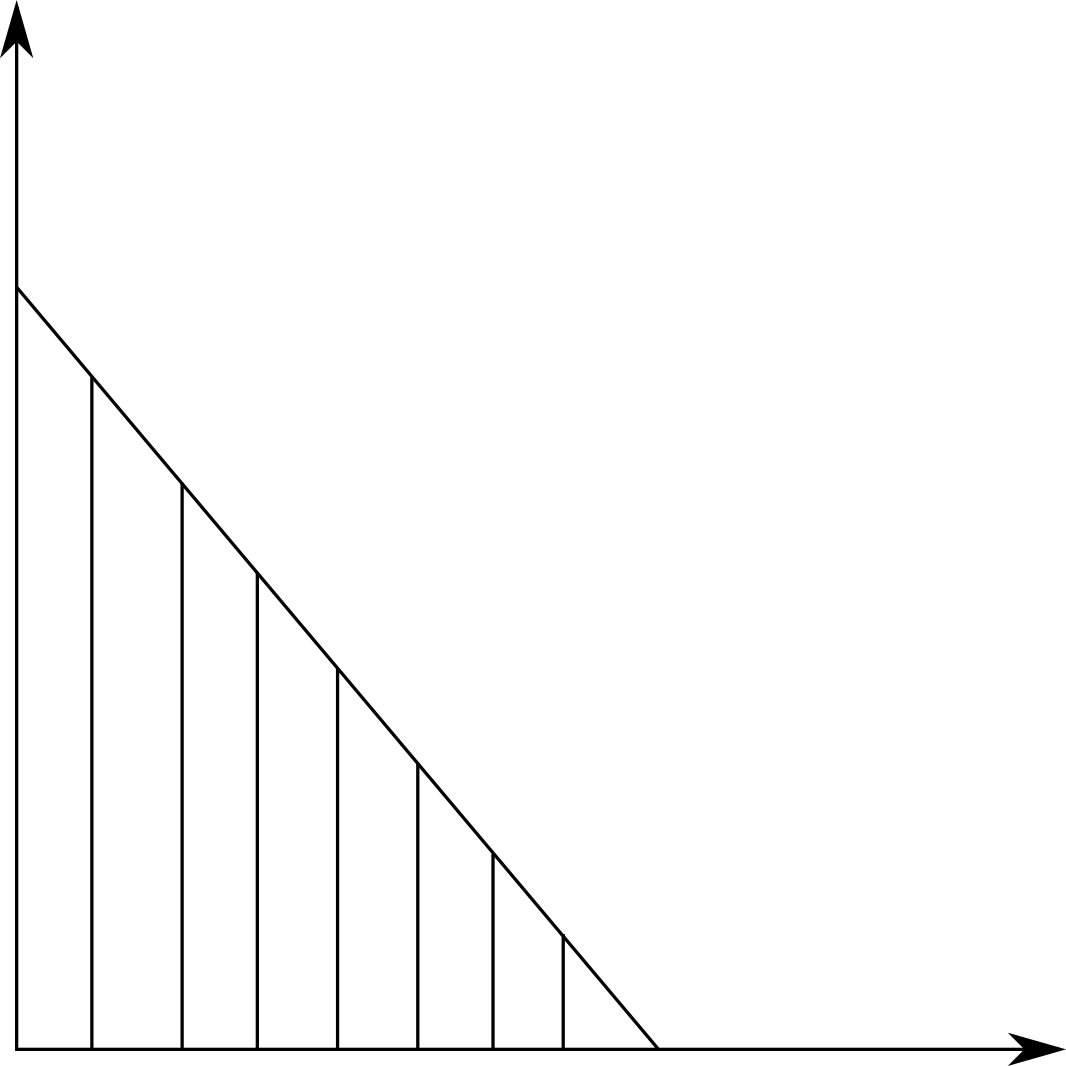
\includegraphics[width=0.5\textwidth]{fig_43}
            \caption{życie było by proste gdybyśmy mogli tak robić}
        \end{figure}
        \[
            \int_{A}f = \int_0^1 dx \int_0^1 dy f(x,y) \overset{\text{?}}{=} \int_0^1dy \int_0^1dx f(x,y)
        .\]
    \end{przyklad}
    \begin{tw}
        (Fubiniego)\\
        Niech $f: A\times B\to \mathbb{R}$. $A\subset\mathbb{R}^l, B\subset\mathbb{R}^k, A\times B\subset\mathbb{R}^n$, $f$ - ograniczona i całkowalna na $A\times B$. Oznaczmy $x^l\in A, y^k\in B$, $A,B$ - kostki.\\
        Niech \[
            \varphi(x) = \overline{\int_B}f(x^l,y^k)dy^k, \psi(x) = \underline{\int_B} f(x^l, y^k)dy^k
        .\]
        Wówczas \[
        \int_{A\times B} f = \int_A \varphi = \int_A \psi
        .\]
        \begin{uwaga}
            całkowalnośc na $A\times B$ nie oznacza całkowalności na np. $B$.
        \end{uwaga}
    \end{tw}
    \begin{dowod}
        Niech $\left\{ Q_i \right\} = \Pi_1$ - podział zbioru $A$, $\left\{ R_j \right\} = \Pi_2$ - podział zbioru $B$.\\
        Wówczas  $\Pi_1 \times \Pi_2$ - podział $A\times B$.
        \begin{align*}
            &\underline{S}(f,\Pi_1\times \Pi_2) = \\
            &= \sum_{\substack{Q_i\\ R_j}} \underset{\substack{x\in Q_i\\ y\in R_j}}{\inf} f(x,y) |Q_i| |R_j| \le\\
            &\sum_{Q_i}\sum_{R_j} \underset{x\in Q_i}{\inf} \underset{y\in R_j}{\inf} f(x,y) |Q_i| |R_j|\le\\
            &\le \sum_{Q_i}\underset{x\in Q_i}{\inf} \underset{\text{suma dolna dla $\psi(x)$}}{\sum_{R_j}\underset{y\in R_j}{\inf} f(x,y) |R_j| |Q_i|}\le\\
            &\le\sum_{Q_i}\underset{\text{bo suma dolna $\le$ całki dolnej}}{\underset{x\in Q_i}{\inf} \psi(x) |Q_i|} = \underset{S}(\psi,\Pi_1)
        .\end{align*}
        Ale $\underline{\int_A}\psi(x) = \underset{\Pi}{\sup} \left| \sum_{Q_i}\underset{x\in Q_i}{\inf} \psi(x) | Q_i | \right|$.\\
        Czyli $\underline{S}(f,\Pi_1\times\Pi_2) \le \underline{S}(\psi,\Pi_1)$. Analogicznie możemy pokazać, że\\
        \[\underline{S}(\psi,\Pi_1)\le\underline{S}(\varphi,\Pi_1)\le\overline{S}(\varphi,\Pi_1) \le\overline{S}(f,\Pi_1\times\Pi_2).\]
        Zatem
        \[
            \underline{S}(f,\Pi_1\times\Pi_2) \le \underline{\underline{S}(\psi,\Pi_1)} \le \overline{S}(\psi, \Pi_1) \le \underline{\overline{S}(\varphi,\Pi_1)} \le \overline{S}(f,\Pi_1\times\Pi_2)
        .\]
        Skoro $f$ - całkowalna na $A\times B$, to
    \[
        \underset{\varepsilon>0}{\forall} .\underset{\Pi}{\exists} |\overline{S}(f,\Pi) - \underline{S}(f,\Pi)|<\varepsilon
    .\]
    Co oznacza, że $\int_A \psi$ i $\int_B \varphi$ - istnieją i wynoszą $\int_{A\times B} f \quad\Box$

    \end{dowod}
\end{document}
